A chronology of key events in the history of Palestine and the development of the Israeli/Palestinian conflict since the 1880s. The political history is detailed to present the reasons for demolishing a large number of Palestinian villages. Focused details about Al-Ghabisiyya village as a case study. Then the chapter will address the cultural identity of the Palestinian refugees from the perspective of a second and third generation. The last section will explain the first steps of the application development from the \acrshort{yallah!} hackathon exchange program.  
\section{Political History}

Palestine, a nation known for decades to have existed in political conflict. In the 1880s, Zionist immigration to Palestine began with the goal of establishing a national home for the Jewish people on their ancient land, Israel, in Zionist words \citep{Morris2004, Pappe2006, Khalidi2015}.

After Basel's first Zionist Congress in 1897, at which the idea of creating a Jewish state in Palestine was first presented, Vienna's rabbis sent two delegates to examine the country's suitability for such an undertaking. 
In this document, the respondents reported to Vienna the results of their explorations:





\centerline{\textit{\say{The bride is beautiful, but she is married to another man.}}}


This document summarized the issue the Zionist movement had to confront from the start, an Arab nation actually living on the land the Jews had set their hopes upon. With the exception of some minority parties, the Zionist movement tended to ignore the existence of Palestinians over the land \citep{Shlaim2014, Karmi2007}.

\say{Zionism secularized and nationalized Judaism. To bring their project to
fruition, the Zionist thinkers claimed the biblical territory and recreated,
indeed reinvented, it as the cradle of their new nationalist movement. As they
saw it, Palestine was occupied by \say{strangers} and had to be repossessed.
\say{Strangers} here meant everyone not Jewish who had been living in Palestine
since the Roman period. For many Zionists Palestine was not even an 
\say{occupied} land when they first arrived there in 1882, but rather an \say{empty} 
one, the native Palestinians who lived there were largely invisible to them or, 
if not, were part of nature's hardship and as such were to be conquered and 
removed. Nothing, neither rocks nor Palestinians, was to stand in the way of 
the national \say{redemption} of the land the Zionist movement coveted} \cite[p.11]{Pappe2006}.


At the very same time, throughout the last decades of the 19$^{th}$ century, the Arab Revolution was emerging to achieve \say{independence} from the Ottoman Empire. Nevertheless, the possibility for a possible Jewish conquest of the state and the displacement of the native Palestinian people was clear to some Palestinian leaders even before the First World War, it was acknowledged in the publications of the founders of Zionism. Historical evidence indicates that between 1905 and 1910, many Palestinian leaders addressed Zionism as a political movement to buy property, and influence in Palestine, although the disruptive aspect was not well understood at the time. \citep{Pappe2006}.



 The British government published a Balfour declaration in 1917 and during the First World War declaring the support for creating a \say{National Home for the Jewish people in Palestine}. The First World War devastated the Ottoman Empire that same year, and Britain captured Palestine \citep{Morris2004}.  
 
 
 
 
 
 The British Mandatory for Palestine was accepted in 1923 and from that year until 1948 Palestine was under the British mandate. The British Mandatory Government officials had permitted the Zionist movement to create its autonomous territory within Palestine with an infrastructure for a future state. By the late 1930s, the Zionist leaders were able to shape the theoretical concept of Jewish permanence into concrete plans \citep{Pappe2006}.  
 
Orde Charles Wingate, an officer of the British Army who made the Zionist leaders understand more thoroughly that the concept of Jewish statehood will have to be strongly associated with militarism and an army, Wingate also became a Zionist and began to train and instruct Jewish settlers techniques of fighting against the native population, in 1920 he founded and created \say{Hagana} \textit{(“Defence” in Hebrew)}, the Jewish community armed group in Palestine. During the Arab revolt against the British Mandate, he succeeded in merging Hagana troops with British forces. The Hagana troops received their first training in 1938 to capture a Palestinian village together with the British forces assaulted a village at the Lebanese border and retained it for hours \citep{Pappe2006}. \say{Moshe Dayan \textit{(an Israeli military leader and politician)}, who said: Wingate had taught us everything we know}\cite [p.112]{Fenby2018}. 

In the Second World War, Hagana has gained valuable combat experience when many of its participants served for the British war effort \citep{Pappe2006}. Irgun and Lehi \textit{(Stern Gang)} two paramilitary groups that came out of Hagana. Irgun split from Hagana in 1931 and Lehi divided from Irgun in 1940\citep{Shlaim2014}. Both groups were seen as terrorist organizations or entities which commits acts of terror against Palestinians and British authorities \citep{Bell1976}.   


The British government released a policy paper entitled \say{The White Paper} in May 1939, promising the inhabitants of Palestine statehood and autonomy within ten years, and restricting Jewish immigration to 75,000 for five years. The White Paper also dismissed the notion of dividing Palestine in order to stop the Arab rebellion that began in 1936 \citep{Morris2004, Fenby2018}.

That wasn't in the Jewish Agency's benefit. The Jewish Agency, therefore, started to consider military intervention as tension mounted to strike the British within the Haganah. The Haganah continued to remain with the British in cooperation. But in 1944, the Irgun and Lehi started a revolt toward British rule. In reaction to British restrictions on immigration, they targeted police and government targets.
Certainly, Lehi(Stern Gang) was determined to fulfill the Zionist dream, so Stern, before he realized that Hitler was exterminating the Jews in Europe, has offered Nazi Germany help and support to fight the British and push them out of Palestine. This initial relationship with Nazi Germany eventually cost Lehi and Stern himself a great deal of support \citep{Shlaim2014, Heller1995, Grob-Fitzgibbon2011}. 

Considering the reality of exterminating the Jews in Nazi Germany concentration camps, Irgun and Lehi intentionally avoided strategic targets to guarantee that the British war effort against their common enemy, Nazi Germany, was not hampered. After the 1945 defeat of Nazi Germany at World War II, the Haganah, Irgun, and Lehi decided to join as the Jewish Resistance Movement, they operated under a joint command formation consisting of members of all three groups and carefully planned their activities. The Haganah also assisted the Irgun command with 460 Palmach warriors (Haganah's elite armed forces) and provided it with funding. Whereas the Irgun and Lehi would continue to pursue a complete-scale rebellion towards the British, the Haganah envisaged a more targeted effort to force the British to adhere to Zionist demands, combining attacks primarily to immigration-related goals \citep{Bell1976, Shlaim2014}.

Notwithstanding the white paper orders, after the Holocaust Jewish illegal immigration to Palestine persisted and increased, the Zionist organizations in Europe set up a well-organized system to immigrate 350,000 Jewish immigrants to Palestine between November 1931 and December 1946.\citep{Grob-Fitzgibbon2011, Heller1995}.   

Lehi and Irgun expanded their terrorist attacks against the British authorities at various locations in Europe and Palestine, exploded the British Embassy in Rome, bombed the British Colonial Club in London, targeted the British 6$^{th}$ Airborne car park in Tel Aviv, destroyed the British police station in Haifa with a truck bomb and exploded the King David hotel \citep{Bell1976}. However the British reacted mildly, particularly when compared to the cruel treatment they conducted on Palestinian revolutionaries in the 1930s \citep{Pappe2006}.
 
 
 
 
\say{The decision was made by the British Cabinet to pull out of Mandatory
Palestine and leave it to the \acrshort{un} to solve the question of its future. The \acrshort{un}
took nine months to deliberate the issue, and then adopted the idea of partitioning
the country. This was accepted by the Zionist leadership who, after
all, championed partition but was rejected by the Arab world and the Palestinian leadership, who instead suggested keeping Palestine a unitary
state and who wanted to solve the situation through a much longer process
of negotiation}\cite[p.40]{Pappe2006}.
 
In the meantime, the Jewish paramilitary received a significant amount of weapons in a secret delivery in April 1948 \citep{Morris2008, Pappe2006}. 
The Haganna leaders formulated the strategy of ethnic cleansing at the beginning of March and it was named Plan D \citep{Shlaim2014}. The strategy targeted at removing every Arab or Palestinian aspect within the country \citep{Pappe2006, Shlaim2014}.
 
Plan D had multiple operations at various dates and different locations:
Nahshon in Jerusalem (2–3 April – 20 April),
Mishmar Ha‘emek (4–15 April),
Ramat Yohanan (12–16 April),
Arab Tiberias (16–18 April), 
Arab Haifa (21–22 April,)
Operation Yiftah, in eastern Galilee (15 April – 15 May), and
Operation Ben-Ami (parts I and II), in western Galilee\citep{Morris2004}.

The British departed on 15 May 1948 and the Jewish Agency proclaimed the creation in Palestine of a Jewish state officially recognized by the two superpowers of the day, the United States and the USSR \citep{Pappe2006}.
 
 According to \cite{Sanbar2007} “1948. That year, a country and its people disappeared from both maps and dictionaries.” \citep{Sanbar2007}. 



The war that led to the establishment of the Israeli state over Palestine in 1948 also contributed to the destruction of the Palestinian nation \citep{Sadi2007}. That day Israel was established over Palestine was a catastrophe for Palestinians \textit{(in Arabic, "Nakba")}. At least 80 percent of the Palestinians living in the territory of Palestine on which Israel was founded became refugees. “The lives of the Palestinians at the individual, community, and national level were dramatically and irreversibly changed” \citep{Sadi2007}.

A huge number of Palestinians were deported outside Palestine during the "Nakba". “Of the
1,400,000 Palestinians in the country prior to the Nakba, just 150,000 individuals were listed
as being present during the first census carried out by the new Israeli state” \citep{Sanbar2007}.



According to \cite{Falah1996}, Some of the terms of Israel's military code are Matate (Broom) and Bi'ur Chametz (Passover Cleanup) indicate that the war contained an element of ethnic cleansing \citep{Falah1996, Pappe2006}. During the 1948 war, Palestinian villages were destroyed and depopulated by Israeli forces, as shown in figure \ref{fig:map}, the red dots represent the demolished villages, and the yellow dots represent the depopulated villages. 
According to the \acrshort{unrwa}, more than 5 million Palestinian refugees were registered in January 2015, divided between, The West Bank, Gaza
Strip, Syria, Lebanon, and Jordan \citep{Khalidi2015, DajaniDaoudi2011}. 

The Palestinian refugees have not been allowed back to Palestine since 1948, and not even for a visit. Because of the idea of returning large numbers of Palestinians to their villages and cities, or even to any part of Palestine, it impacts on Israelis high-seated concerns about the validity and continuity of the whole Zionist system, and also the Arab-Jewish population equation in Palestine \citep{Khalidi2016}.

\begin{wrapfigure}{r}{0.20\textwidth} %this figure will be at the left
    \centering
    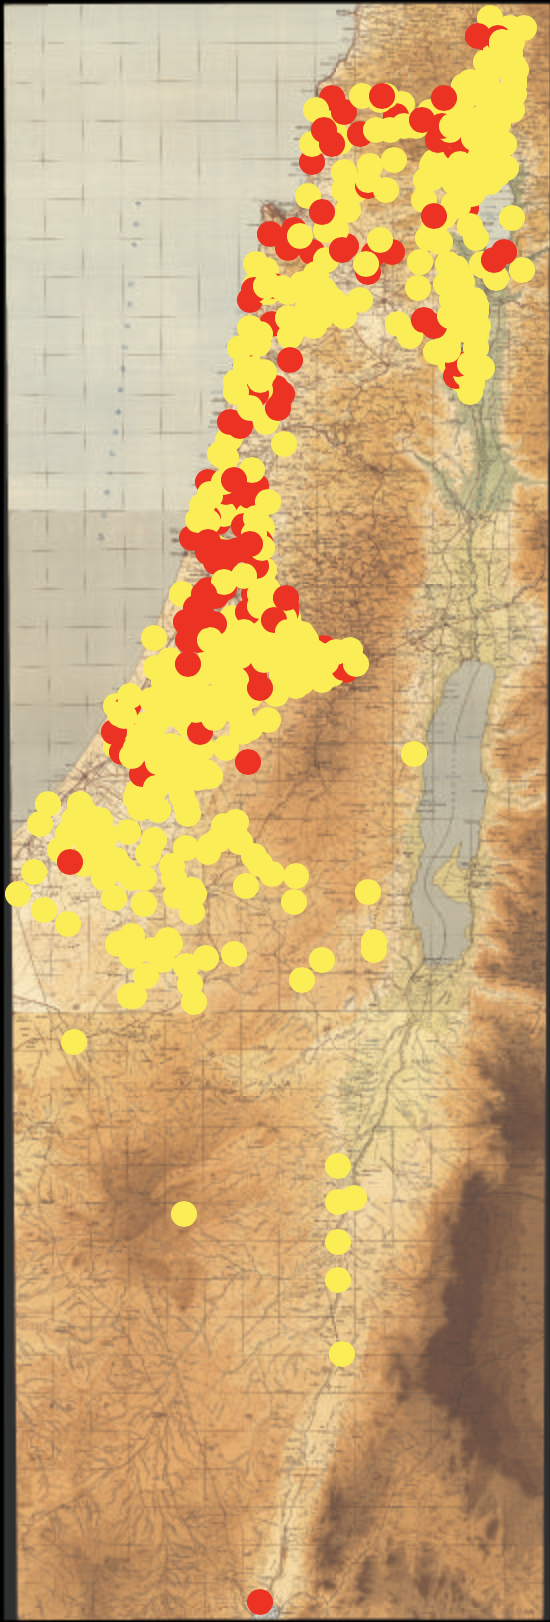
\includegraphics[width=0.20\textwidth]{d_villages}
    \caption{Demolished and depopulated villages - Palestine Open Maps, © 2018  Visualizing Palestine}
    \label{fig:map}
\end{wrapfigure} 

According to Pappé (2006), the Zionist organization and the Hebrew University mapped and made a detailed registry of all the Arab villages \citep{Pappe2006}.



The project of mapping the whole villages details was funded by \textit{\acrfull{jnf}} and turned out to be a \say{national project} and it was called \say{The village files}\citep{Pappe2006}. 


The \say{archive} was nearly complete in the late 1940s and the information became more specifically military-oriented. \citep{Pappe2006}. In 2018 the Israeli national archive was published online, but after a time of research through the archive in English and in Hebrew, those maps and the detailed information about the villages were not openly published. According to Shezaf (2019), The Secret Security Department (Malmab) of the Israeli Defense Ministry is responsible for concealing hundreds of documents as part of a concerted effort to conceal Nakba evidence \citep{Shezaf2019}.\say{Yehiel Horev, who headed Malmab for two decades, until 2007,
acknowledged to Haaretz that he launched the project, which is still
ongoing. He maintains that it makes sense to conceal the events of
1948, because uncovering them could generate unrest among the
country’s Arab population. Asked what the point is of removing
documents that have already been published, he explained that the
objective is to undermine the credibility of studies about the history
of the refugee problem}\citep{Shezaf2019}.


\subsection{Operation Ben-Ami}

Around 13 and 22 May 1948, Operation Ben-Ami was explicitly told in two phases that the villages had to be destroyed in retaliation for the convoy's defeat. Therefore the villages of Sumiriyya, Zib, Bassa, Kabri, Umm al-Faraj, and Nahr are exposed to an expanded, more brutal form of the Israeli force's \say{destroy-and-expel} exercise. They aimed to invade, execute, destroy and set fire to Kabri, Umm al-Faraj, and Nahr for the sake of occupation \citep{Pappe2006}. The operation aimed for capturing and clearing all the villages along the coast from the south of Acre to Ras Al-naqoura in the north by the Lebanese borders \citep{Morris2004, Morris2008}.

Part of the Haganna troops arrived with armored vehicles and some troops arrived by boat near Sumiriyya, the Haganna men went through the coast and they attacked Sumiriyya with mortars and left the eastern side open so that inhabitants could flee. \citep{Morris2004, Morris2008}.

Bassa took over a day to defeat because of the village militant's resistance and some volunteers from the \textit{\acrfull{ala}}. The resistance gave the Haganna another incitement to \say{punish} the village further than the expulsion of their people. Haganna troops stormed Bassa and demanded all the young men in front of one of the churches to be lined and then executed them. The last village that collapsed in phase two of the Ben-Ami campaign after the massacre was Al-Ghabisiyya \citep{Morris2004, Pappe2006}.  



\section{Al-Ghabisiyya Village}

Al-Ghabisiyya is 11.5 km north-east of the Acre. The village sat on a rocky heap rising from the Acre plain. The site was probably a large Canaanite town, extrapolating from the many caves that were used as tomb places.
Al-Ghabisiyya had 690 residents and, 125 houses in 1931. Built in the late 19th century, the village was populated by 150 people at the time \citep{Khalidi2015}.
\subsection{Al-Ghabisiyya before 1948}

 Al-Ghabisiyya has been surrounded by a wide range of trees such as olives, figs, and pomegranate. The village was close to Shaykh Dannun and Shaykh Dawud's other two villages. Shaykh Dawud and Shaykh Dannun were intersected at places, but they were only 500 meters away from Al Ghabisiyya. These villages total population was Muslim. 

The Ottomans had founded and built a school at Al-Ghabisiyya in 1886. The buildings of the village are constructed of reinforced concrete and in some situations, the rock kept together with mud or cement mortar. The village's economy is dependent on livestock farming, and the main harvests were grains, and vegetables. The villagers also cultivate olives and pressed it in two animal-drawn presses, one was in Al-Ghabissya and the other in Shaykh Dawud.

A total of 6633 dunums were distributed for grains from the lands of the three villages in 1944/45, 1371 dunums were replanted or used for fruit trees. That year, 300 dunums were committed to olive trees in Al-Ghabisyya \citep{Khalidi2015}.

\subsection{Occupation and Depopulation}

At the end of Operation Ben-Ami, the Haganah's invasion of Palestine's northwest corner, Al-Ghabisiyya fell. The operation, which started from 13 to 14 May 1948, was the last major Haganah offensive in Palestine before the end of the British Mandate \citep{Khalidi2015}.

In the words of the Israeli historian Benny Morris, \say{This was in line with Plan D provision for securing blocks of Jewish settlement even outside the partition plan borders} \cite[p.252]{Morris2004}.

The order was given to the Carmeli Brigade that carried out the operation on 19 May 1948, "to attack with the aim of conquest, the killing of adult males, destruction and torching villages of Al-Kabri, Umm al Faraj and Al-Nahr" \cite[p.253]{Morris2004}. The following night, 20-21 May, Al-Kabri was occupied as part of the second phase of Ben-Ami operation. Al-Nahr was captured during this second stage of the operation, along with several villages in western Galilee, north of Acre, between 20-21 May 1948. Carmeli Brigade units targeted Al-Ghabisiyya on the same date being the last village to be taken. Al-Ghabisiyya officially fell, the residents received the troops with white flags, but Carmeli's troops shot some residents and then executed six more \citep{Morris2008}. Most of its inhabitants were deported in the days or even weeks that followed \citep{Morris2004}.

From two locations, north and southeast, the attacks were carried out. The invading forces seized a home in the village's southernmost area, shelling the village out of the house, killing and wounding many of the civilians as they fled. The village militia preferred not even to fight the Zionist forces as they were too few (about twenty) and equipped very poorly. Most of those who were driven out remained in other villages in Galilee until the whole region fell at the end of October 1948, after that they were displaced to Lebanon \citep{Khalidi2015}.

Several people stayed until February 1949 in Al-Ghabisiyya. This time, a second expulsion by the military government took place during the same month on the pretext of \say{safety and order}, it's not clear where the villagers were expelled \citep{Morris2004}.

After the evacuation of Al-Ghabisiyya and its two adjacent villages of Shaykh Dannun and Shaykh Dawud, some of the residents of the other two villages were allowed by the Israeli government to return home. Just several families from Al-Ghabisiyya, Al-Nahr, Al-Tall, Umm Al-Faraj, Amqa, and Kuwaykat joined those who had not found refuge in Lebanon. Shaykh Dannun and Shaykh Dawud's two tiny villages were incorporated into a single village called Shaykh Dannun, with a population of about 1000 in 1973. The Al-Ghabisiyya village has not been repopulated \citep{Khalidi2015}.  

\subsection{The Village Today}

The only surviving landmark is the mosque, a building of brick a dome mounted above it, with arched doors and windows and internal elaborate arches. It's abandoned, the concrete plaster on the dome peels off, and the rest of the roof is covered by wild shrubs. It is easy to see the ruins of buildings, terraces, and the village cemetery among a thick forest of pine trees planted on the village site and most of the property. Netiv ha-Shayyara's settlement, implemented in 1950 by Iraqi Jewish immigrants, uses the nearby non-forest land for farming \citep{Khalidi2015}.    
\section{Current Political Context}

The West Bank and East Jerusalem became part of the Kingdom of Jordan after 1948 and the Gaza Strip became an Egyptian area of trust \citep{Houdaille2010}. Israel captured the whole of Palestine in 1967 and also Egypt's Sinai, and Syria's Golan Heights by a six-day battle. The Palestinian Resistance movements united under the name of Palestine Liberation Organization (PLO). The national uprising (in Arabic: intifada) started inside Palestine against the occupation in 1987, where it led to peace negotiations between Yitzhak Rabin representing the Israeli government and Yasser Arafat as a representative of the PLO in 1993. The Oslo Accords is the name of the negotiation between the Israeli government and the PLO, the Oslo Accords are focused on UN Security Council Resolution 242 recommending Israel's departure from the 1967 borders and the Palestinian people's right to self-determination. It was the expectation that a Palestinian state would be created since the Palestinians took control of some cities and lands from the West Bank and Gaza. But due to the Israeli policy of occupying more lands in the West Bank and committing violations of human rights on Palestinians that led to a second uprising (Intifada) in the year 2000 \citep{Shalhoub-Kevorkian2006}. The current situation in Palestine is a very controlled movement for Palestinians, a military checkpoint on every city entrance, and all the Palestinian areas are surrounded by a so-called separation wall. The separation wall is 3 times as long and twice the height of the Berlin wall \citep{Shalhoub-Kevorkian2006}.



\section{Cultural Identity}
 
The expulsion of the 1948 Palestinian village people did not affect a transient population, but an ancient ancestral farming community that belonged to a civilization that elevated the human culture with its connection to religion, literature, art, architecture, and science. Therefore, it is not impossible to imagine the intensity and toughness of the suffering which impacted the families that were displaced in 1948 or why their mental state was transferred in their diaspora to their grandchildren \citep{Khalidi2015}.
 
 The children have grown up fascinated by their relatives and grandparents tales of their abandoned homes and villages and the perfect view of the Palestinian environment and scenery they were forced to leave it behind them and flee.

They see they belong to Palestine through a fight for equality and equal rights for under-occupation Palestinians. The Palestinian connection has been turned into a bond that is more formal but critical. The bond that could be considered as Long-distance post-nationalism. The ongoing violence perpetrated on Palestinians has caused long-distance post-nationalism in the first place. That is the reaction to this abuse and inequality that is enhancing their engagement with their ancestral home country. It's not just about Palestine as the location of origin, it's more about Palestine as a cause. While the point of interaction with Palestine starts with a personal interest and personal story in many instances, it changes the engagement with Palestine from one that can be read nationally to one that can be viewed as entering a fight for equality in more general terms.
The degree to which long-distance post-nationalism will coexist with national ways of belonging in national politics can be hypothesized. Although many of the study researchers in the second generation sympathized with the Palestinian struggle for independence, none of them understood their connection to Palestine by direct involvement in nationalist movements or saw themselves as being reflected by the Palestinian Authority. Nevertheless, it is important to recognize how these various forms of connection are not inherently exclusive and may intersect with one another \citep{Blachnicka-Ciacek2018}.

It is necessary to see how the new post-nationalist conceptualization of Palestine by the second generation could have the ability to universalize the Palestinian struggle and, accordingly, make it inclusive and reachable to those Palestinians who may have felt distanced from their parent home country \citep{Blachnicka-Ciacek2018}. 

\section{The YALLAH! Hackathon}

\acrshort{yallah!} Is a student’s exchange research program between the University of Siegen in
Germany and Birzeit University in Palestine funded by the DAAD. The program was
constructed for a collaboration between students to create social innovation projects.
In \acrshort{yallah!} 2018 there were three different projects Mobile Makerspace, \acrshort{vr} Experience and
\acrshort{yallah!} Computer Club. The \acrshort{yallah!} program is divided into three phases: The preparation
phase (Bootcamp), a research phase in Germany, and an implementation phase in Palestine.
The \acrshort{yallah!} Hackathon preparation phase
the participants of \acrshort{yallah!} learned about some research methods and how to apply them in
the projects through a boot camp week. During the boot camp, the teams took their first
steps in the projects by planning the research track, setting a research question, and building
a strategy to achieve their goals.
The Palestinian and the German students attended the boot camp separately, therefore the
boot camp took a place once in Germany and another time in Palestine. The purpose of the
boot camp was to introduce and train the participants on the research methods (such as how
to make interviews, how to take field notes, and how to observe while working in the field).
The students split up into 3 groups each group studied one method through literature and
then presented it to the other participants. By the end of the presentation, the students
discussed the method together and practiced it inside the group. The boot camp was a very
good practice for the methods and emphasized the research skills of the participants. At the
boot camp in Germany, the Virtual reality project students made their first test in filming with
a 360o camera, they used the Samsung Gear 360 camera to record part of the boot camp
sessions in a purpose to use it later in the project as a testing video. Due to the average video
quality of the Samsung Gear 360 camera, the \acrshort{vr} students added a task to their list that is to
find a 360$^{\circ}$ camera with better quality. The students also discussed the interesting spots in
Palestine related to the historical and religious places mentioned in biblical stories.
The \acrshort{yallah!} Hackathon research phase
The Palestinian students visited Germany for the research phase. The Palestinian and the
German exchange students met in Siegen, Germany for the first time. The students gathered
on the first day and had an introduction from the supervisors about the whole \acrshort{yallah!}
program in general and the research phase in Germany. After the introduction on the first
day, the teams of each project gathered and discussed their plans for the research and the
implementation phases. The \acrshort{vr} team members discussed the kind of methods to be used in
the research, the team decided on Interviews and Thinking Aloud as methods for collecting
data from random people and from Palestinians who live in Germany. Therefore, multiple tasks needed to be done by the team to start working with those methods. The \acrshort{vr}
team split the tasks among the members: creating the interview questions guideline,
documentation, building a prototype, and logistics, for instance, to create a contact list of
interesting people to contact and have an interview with them.
After one month after the end of the research phase, the \acrshort{vr} team had their second gathering
in Palestine to start the implementation phase. The implementation phase contained a lot of
filming in different places in Palestine. Depending on the research results and the discussion
with the team members, they created an organized plan for visiting different places in
Palestine and capturing the area using the camera. The plan included the main cities of
Palestine, famous touristic sightseeing locations and religious places since people showed
high interest to see those spots. Therefore, the team recorded in Jerusalem, Jaffa, Haifa, Acre, Ramallah, Nablus, Jericho, Hebron, and Bethlehem.

\subsection{VR Application development}

During the \acrshort{yallah!} Hackathon trip the development on the \acrshort{vr} application faced a lot of challenges. It was challenging at the development level due to limited experience in \acrshort{vr} technology for the team. In Palestine, the challenges were more complicated and on different levels. The team faced difficulties in movement between cities, due to Israeli military checkpoints between the Palestinian cities. The checkpoints also exist between the Israeli areas and the Palestinian territories that are surrounded by the separation wall as well. Therefore, it reduced the recording time due to the traffic caused by checkpoints, the team couldn't film all the areas to avoid facing problems with the Israeli forces if they interpret filming as a threat for their security. Filming in touristic areas, wasn’t easy since there was a lot of tourists and the camera was standing on a unipod we had to stay around it to avoid it from falling. Al-Aqsa mosque wasn’t easy to film because it is open for tourists only for specific times, and the tourists can’t go inside the Mosque. Since only Muslims are allowed inside the mosque, the camera was taken by a Muslim student from the team and filmed inside the mosque. But there was an unfortunate event, and the camera fell on one of the lenses and gave a blurry picture. The team had the Samsung Gear 360 camera as a backup, and then it was used to film the whole mosque again. On the application development, Unity game engine had some downsides, it was a heavy weighted environment to develop on it a \acrshort{vr} platform, some computers didn’t handle it. But the team managed to work with it on a workstation. They arranged a workstation that could handle the \acrshort{vr} environment on Unity and the workstation had a good quality graphics card that was able to process all the graphics data in Unity. The other challenge was combining, editing and rendering the 360$^{\circ}$ videos. The high-quality videos that were recorded by the GoPro Fusion camera took a big capacity on the hard drives. First, the camera had two lenses, and each lens records a video on a different memory card. Therefore, the videos needed to be combined and after that processed. It was a team effort for solving this task it took a lot of time and computer power. The size of the16 videos was very big and the internet in Palestine was not good enough for uploading such videos over the Internet. Nevertheless, the application was not ready, it didn't have a \acrfull{ui} that would allow the user to navigate between the locations and cities. 
